\subsection{Bauformen von FDM Druckern}
\begin{itemize}
  \item Karthesisch
  \item CoreXY
  \item Delta
  \item Polar
  \item Hangprinter
\end{itemize}


\newpage % ==================================================================

\begin{figure}[ht]
  \subsubsection{Karthesisch}
  % \section{Sensor - Varianten}
  % \subsection{Andere Ansätze fürs Bedleveling}


\adjustbox{valign=t}{\begin{minipage}[t]{0.45\textwidth}
\begin{framed}
  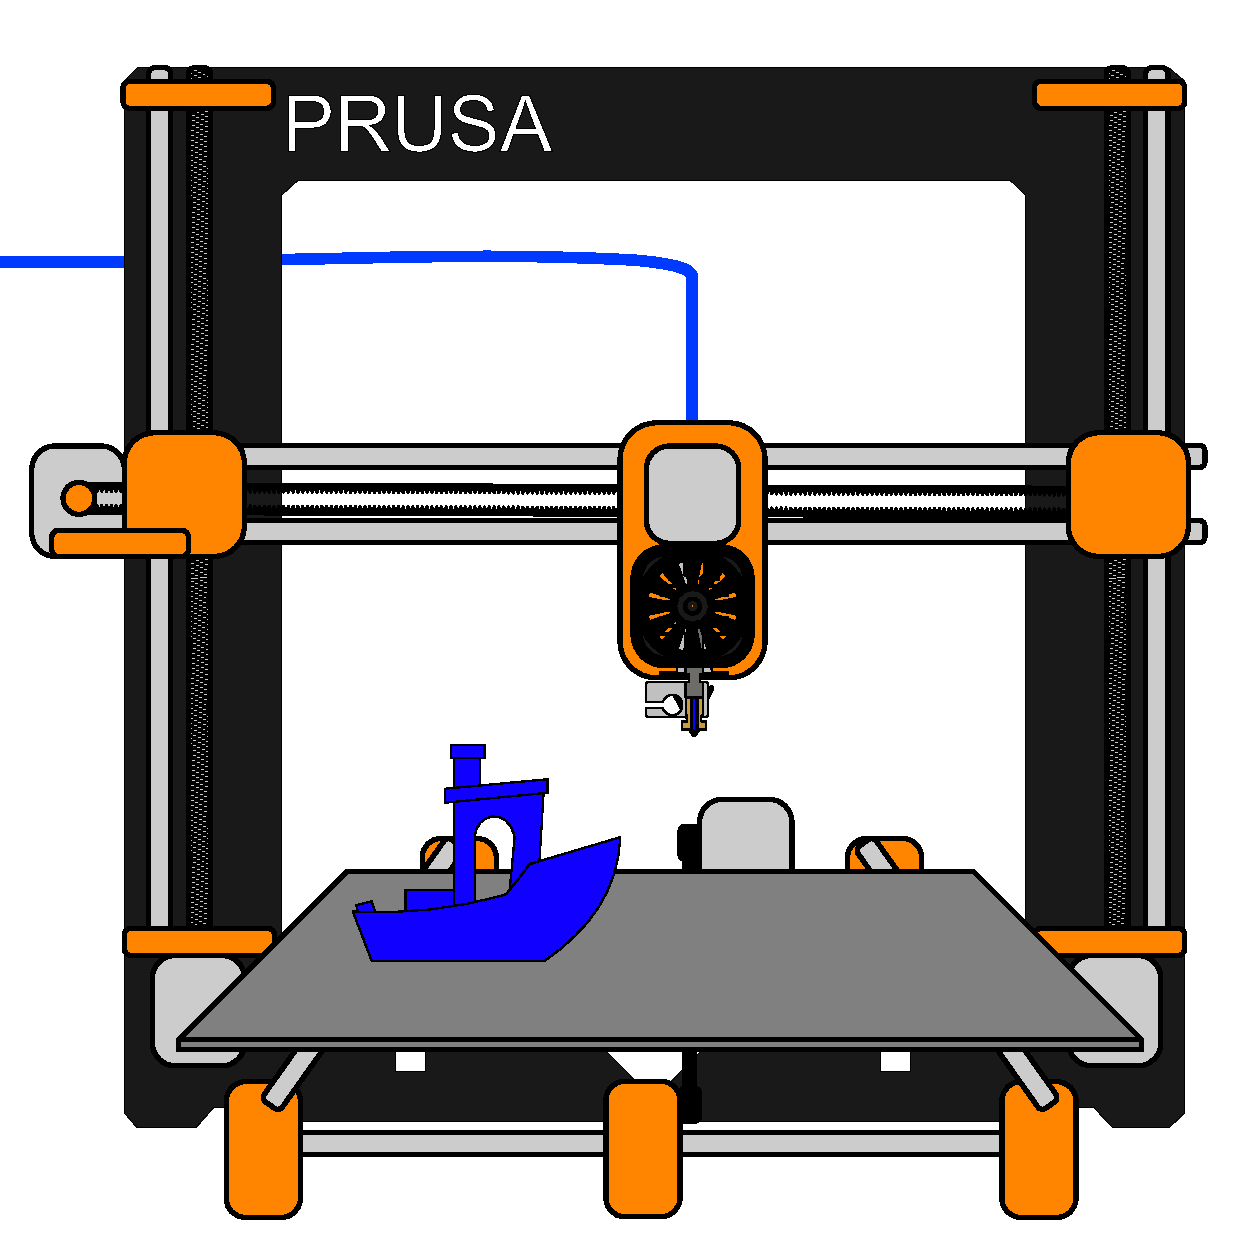
\includegraphics[width=1.0\textwidth, trim = 0px 0px 0px 0px, clip]{./bilder/karthesian.pdf}
\end{framed}

\end{minipage}}
% \hfill
\adjustbox{valign=t}{\begin{minipage}[t]{0.50\textwidth}
\vspace{0pt}
\huge
\hfill{}\textbf{karthesischer Drucker}\\

(Vom Prinzip her auch ein \\
karthesischer Drucker) \\

\vspace{0.2cm}

\textbf{Vorteile:}
\begin{itemize}
  \item Einfach zu bauen.
  \item Fehlerquellen relativ einfach zu finden.
\end{itemize}
\textbf{Nachteile:}
\begin{itemize}
  \item Layershifting
  \item Bei i3 Bauweise bewegendes Druckbed.
\end{itemize}
\end{minipage}}
\end{figure}
\clearpage % GleitObjekte anzeigen





% \subsubsection{Karthesisch}
% \begin{center}
%   \vspace{-2cm}
%   \hfill{}
%   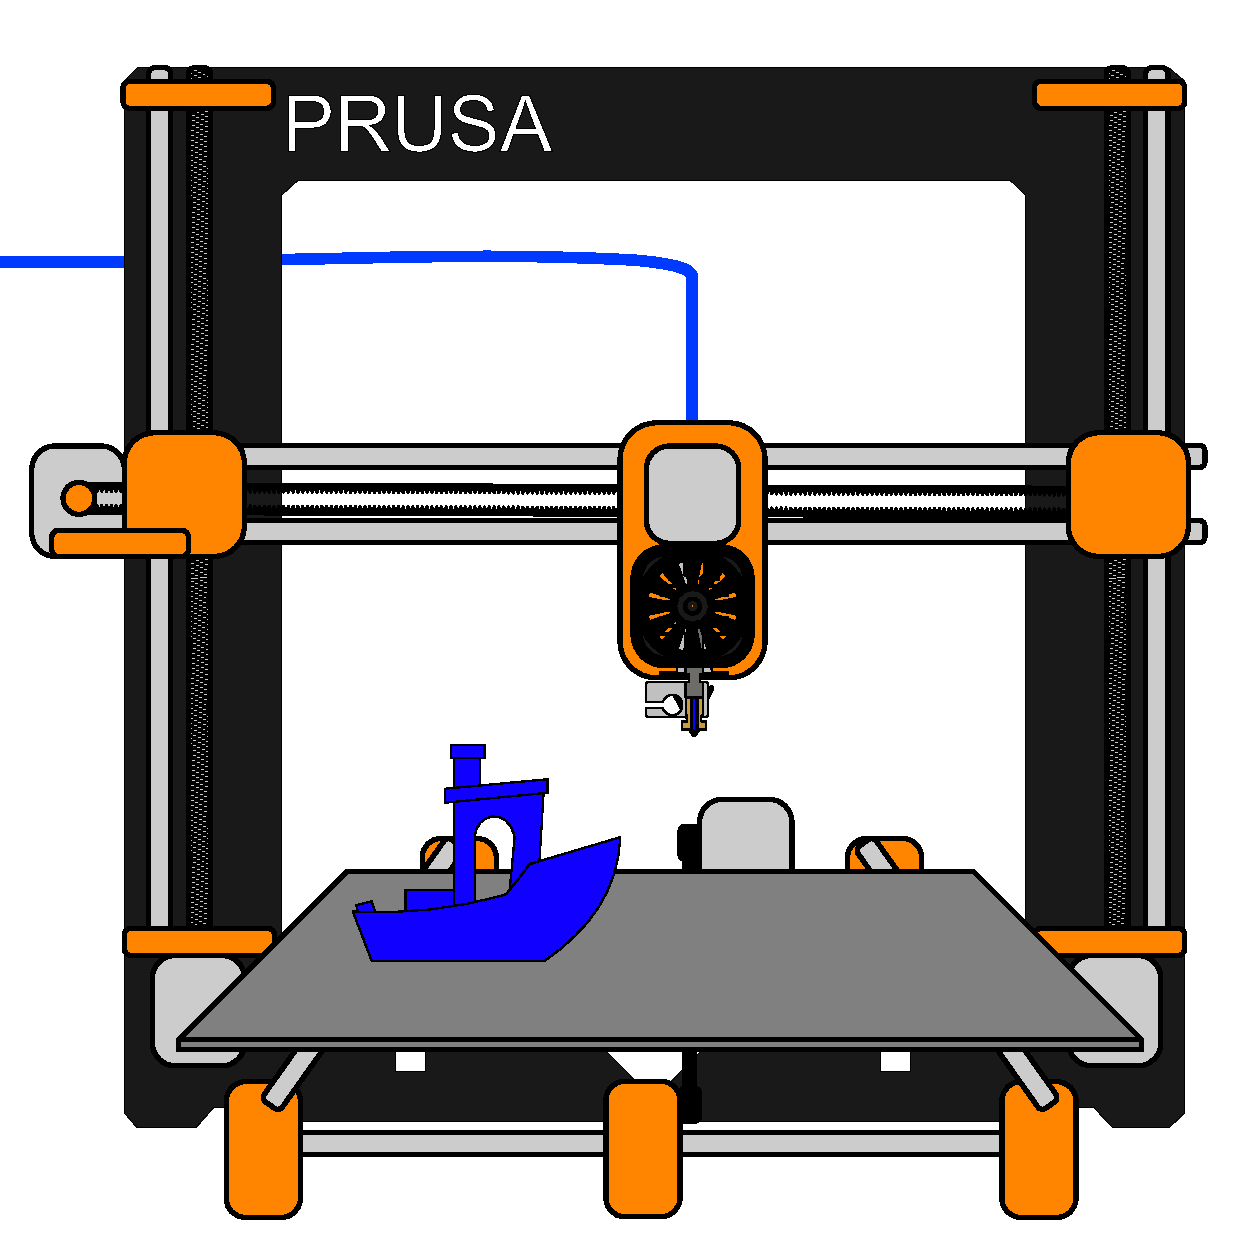
\includegraphics[width=0.4\textwidth]{./bilder/karthesian.pdf}
% \end{center}
% Vorteile:
% \begin{itemize}
%   \item Einfach zu bauen.
%   \item Fehlerquellen relativ einfach zu finden.
% \end{itemize}
% Nachteile:
% \begin{itemize}
%   \item Layershifting
%   \item Bei i3 Bauweise bewegendes Druckbed.
% \end{itemize}

\newpage % ==================================================================

\begin{figure}[ht]
  \subsubsection{CoreXY}
  % \section{Sensor - Varianten}
  % \subsection{Andere Ansätze fürs Bedleveling}


\adjustbox{valign=t}{\begin{minipage}[t]{0.45\textwidth}
\begin{framed}
  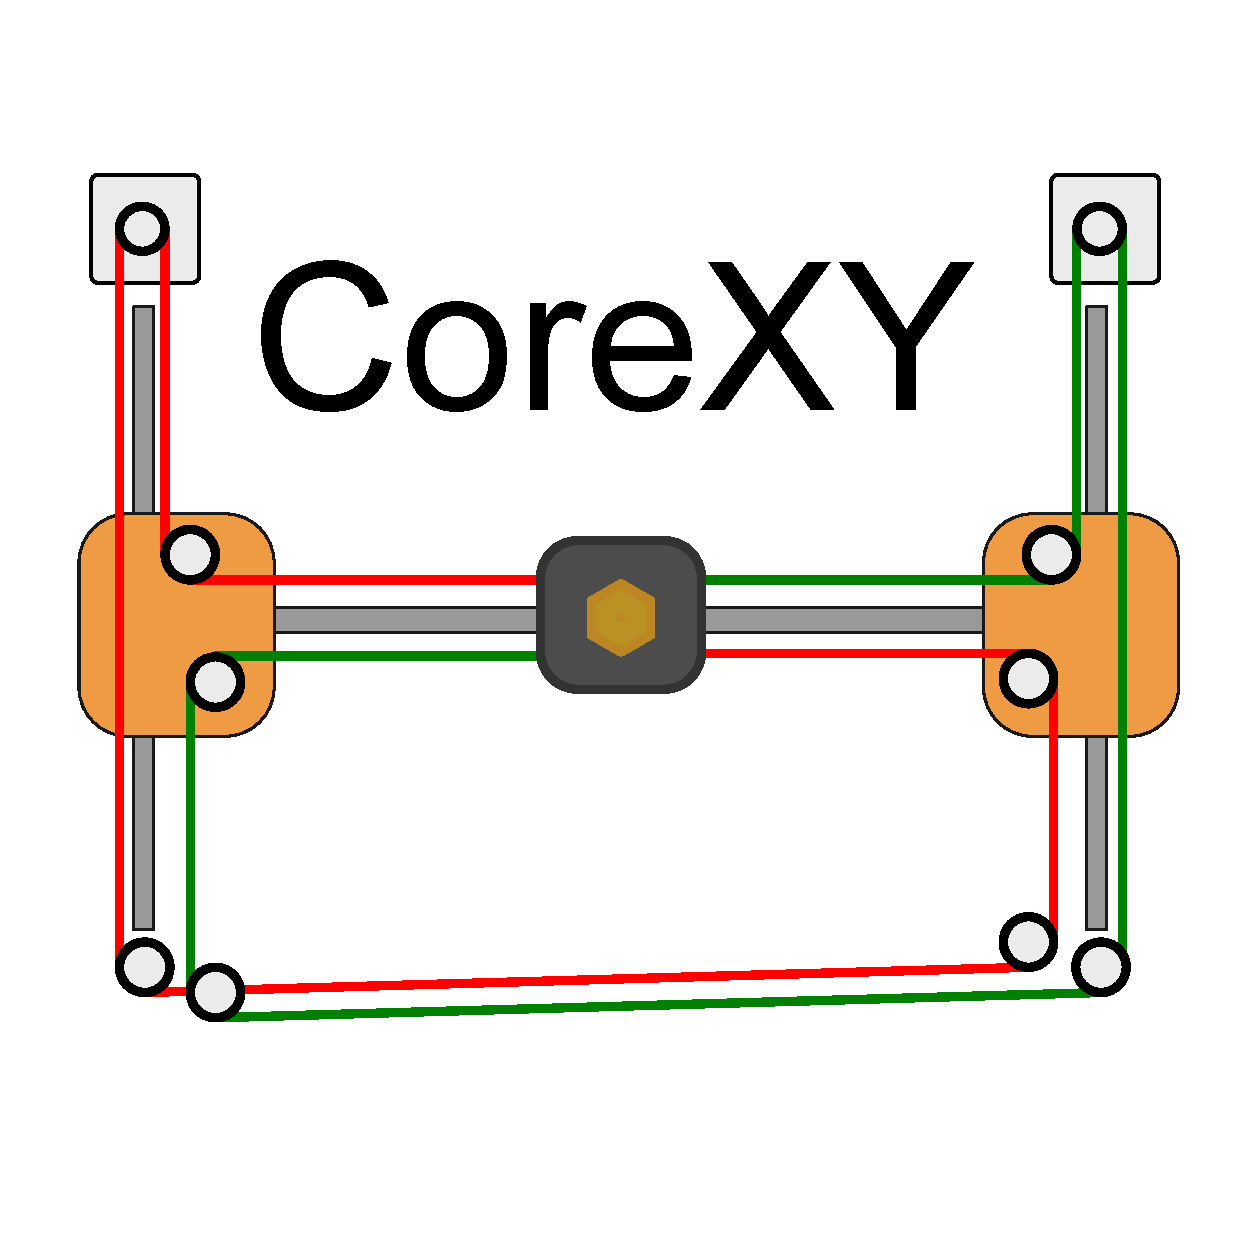
\includegraphics[width=1.0\textwidth, trim = 0px 0px 0px 0px, clip]{./bilder/CoreXY.pdf}
\end{framed}

\end{minipage}}
% \hfill
\adjustbox{valign=t}{\begin{minipage}[t]{0.50\textwidth}
\vspace{0pt}
\huge
\hfill{}\textbf{CoreXY - Drucker}\\

(Vom Prinzip her auch ein \\
karthesischer Drucker) \\

\vspace{0.2cm}

\textbf{Vorteile:}
\begin{itemize}
  \item Relativ einfach zu bauen.
  \item Fehlerquellen (relativ) einfach zu finden.
  \item Festes Druckbed \\$\Rightarrow$ bewegt sich nur in Z Achse.
\end{itemize}
\textbf{Nachteile:}
\begin{itemize}
  \item Layershifting
\end{itemize}
\end{minipage}}
\end{figure}
\clearpage % GleitObjekte anzeigen


% \subsubsection{CoreXY}
% \begin{center}
%   \vspace{-4cm}
%   \hfill{}
%   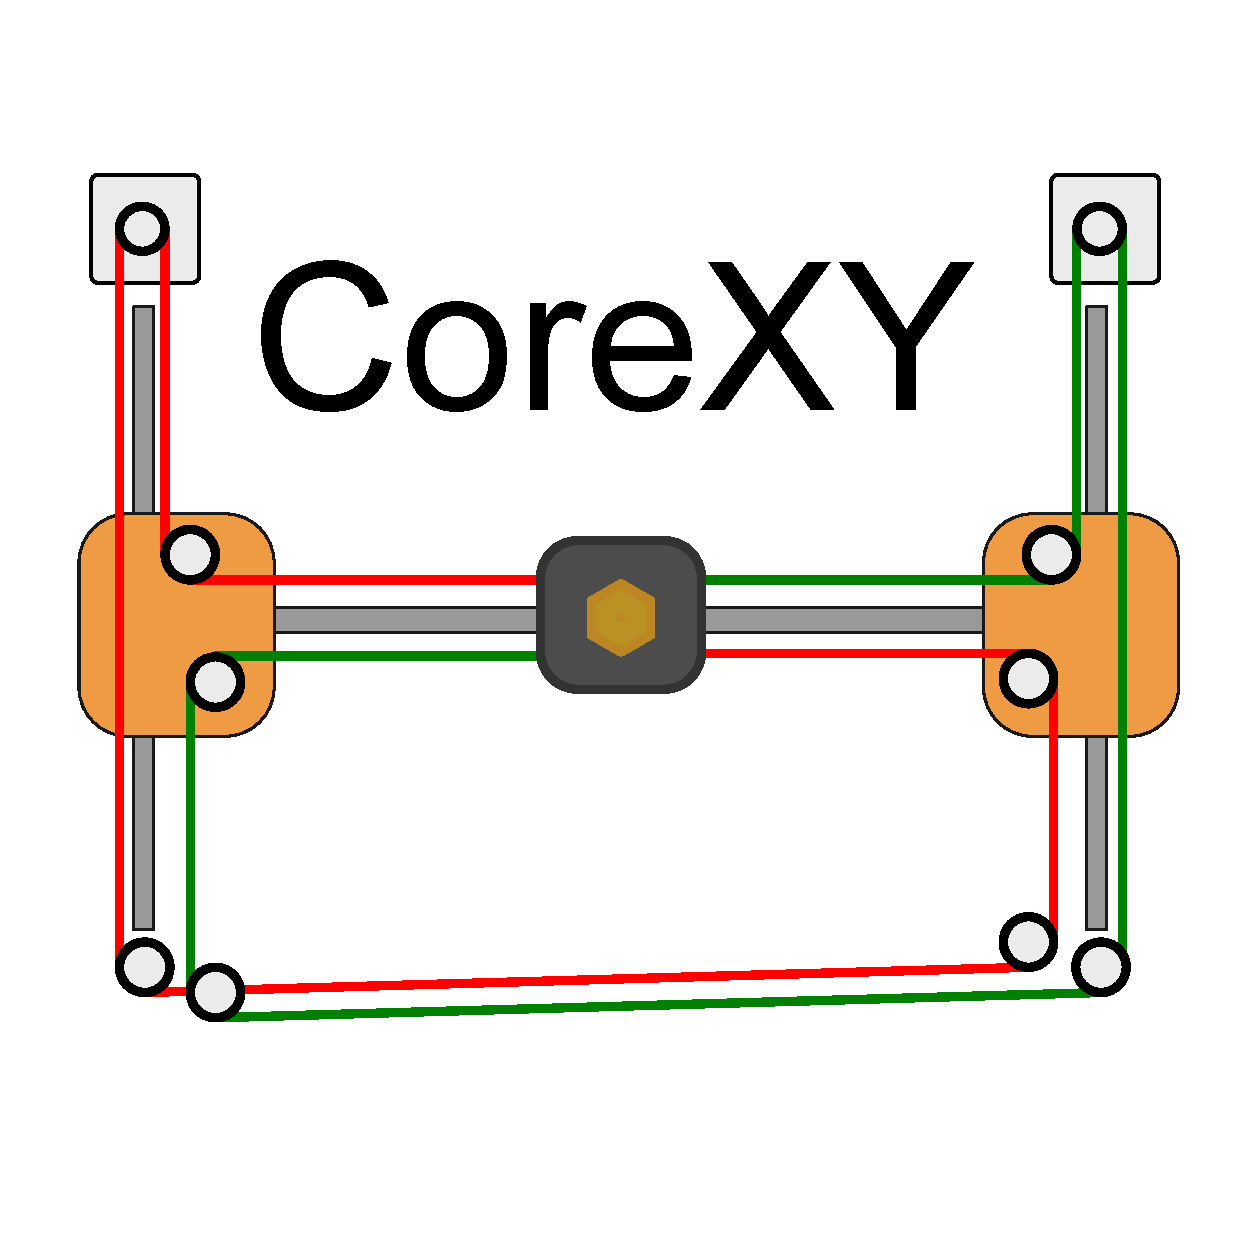
\includegraphics[width=0.5\textwidth]{./bilder/CoreXY.pdf}
% \end{center}
%
% (Vom Prinzip her auch ein karthesischer Drucker)
% Vorteile:
% \begin{itemize}
%   \item Relativ einfach zu bauen.
%   \item Fehlerquellen (relativ) einfach zu finden.
%   \item Festes Druckbed $\Rightarrow $bewegt sich nur in Z Achse.
% \end{itemize}
% Nachteile:
% \begin{itemize}
%   \item Layershifting
% \end{itemize}

\newpage % ==================================================================

% \subsubsection{Delta}
% \begin{center}
%   \vspace{-3cm}
%   \hfill{}
%   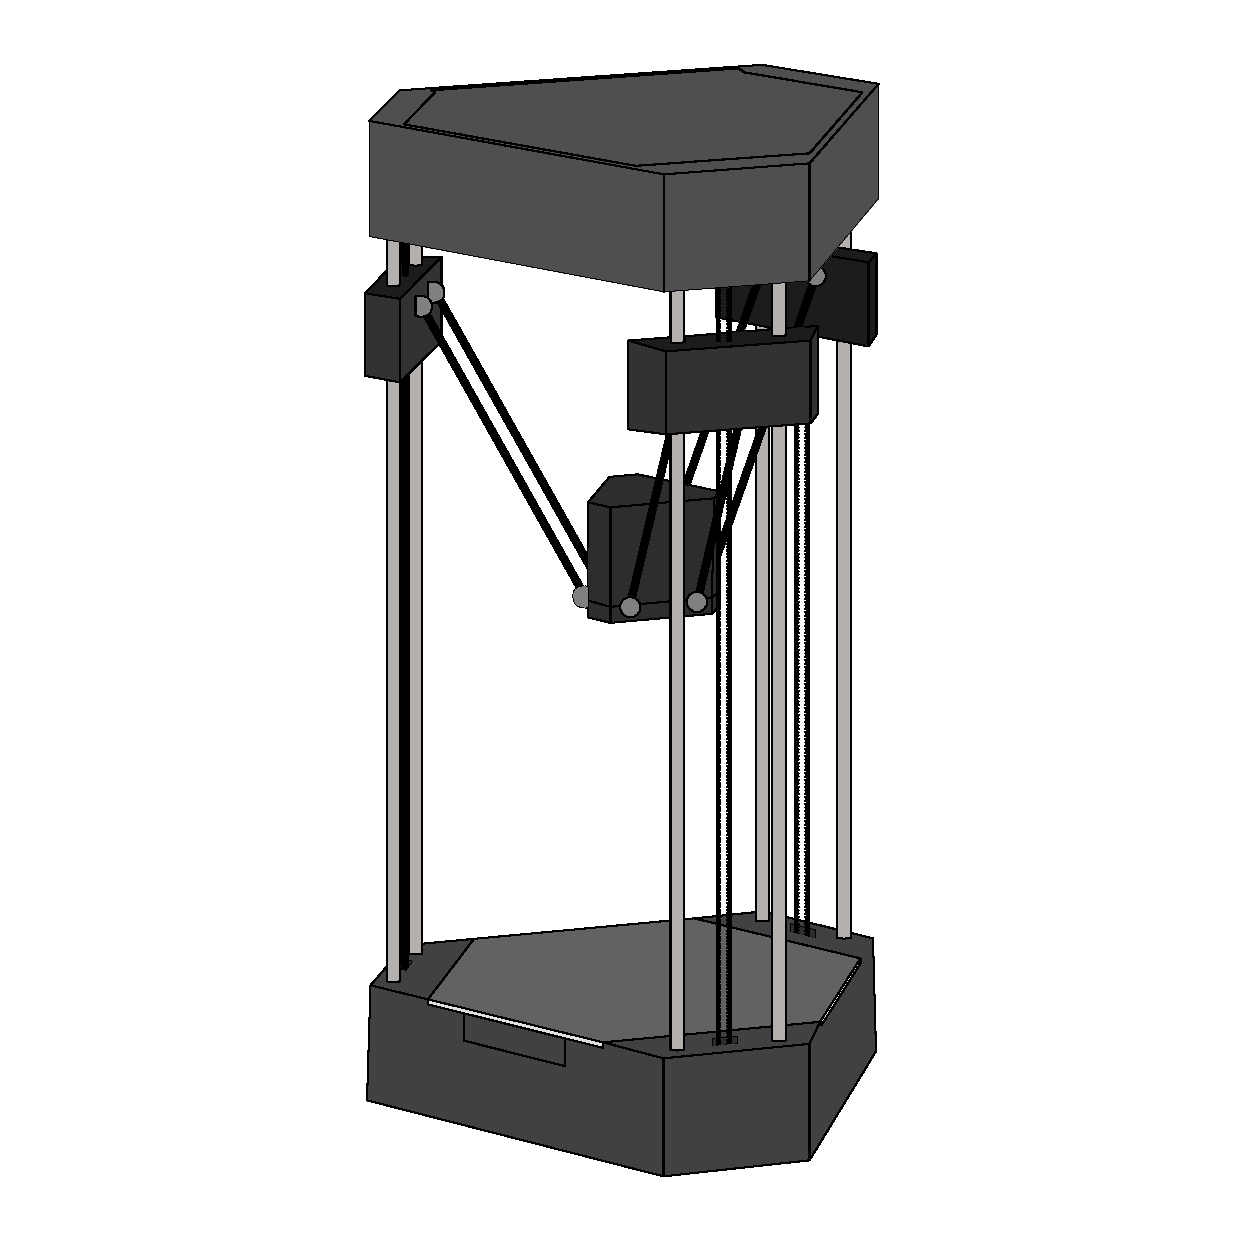
\includegraphics[width=0.5\textwidth]{./bilder/FLUXX.pdf}
% \end{center}

\begin{figure}[ht]
  \subsubsection{Delta}
  % \section{Sensor - Varianten}
  % \subsection{Andere Ansätze fürs Bedleveling}


\adjustbox{valign=t}{\begin{minipage}[t]{0.45\textwidth}
\begin{framed}
  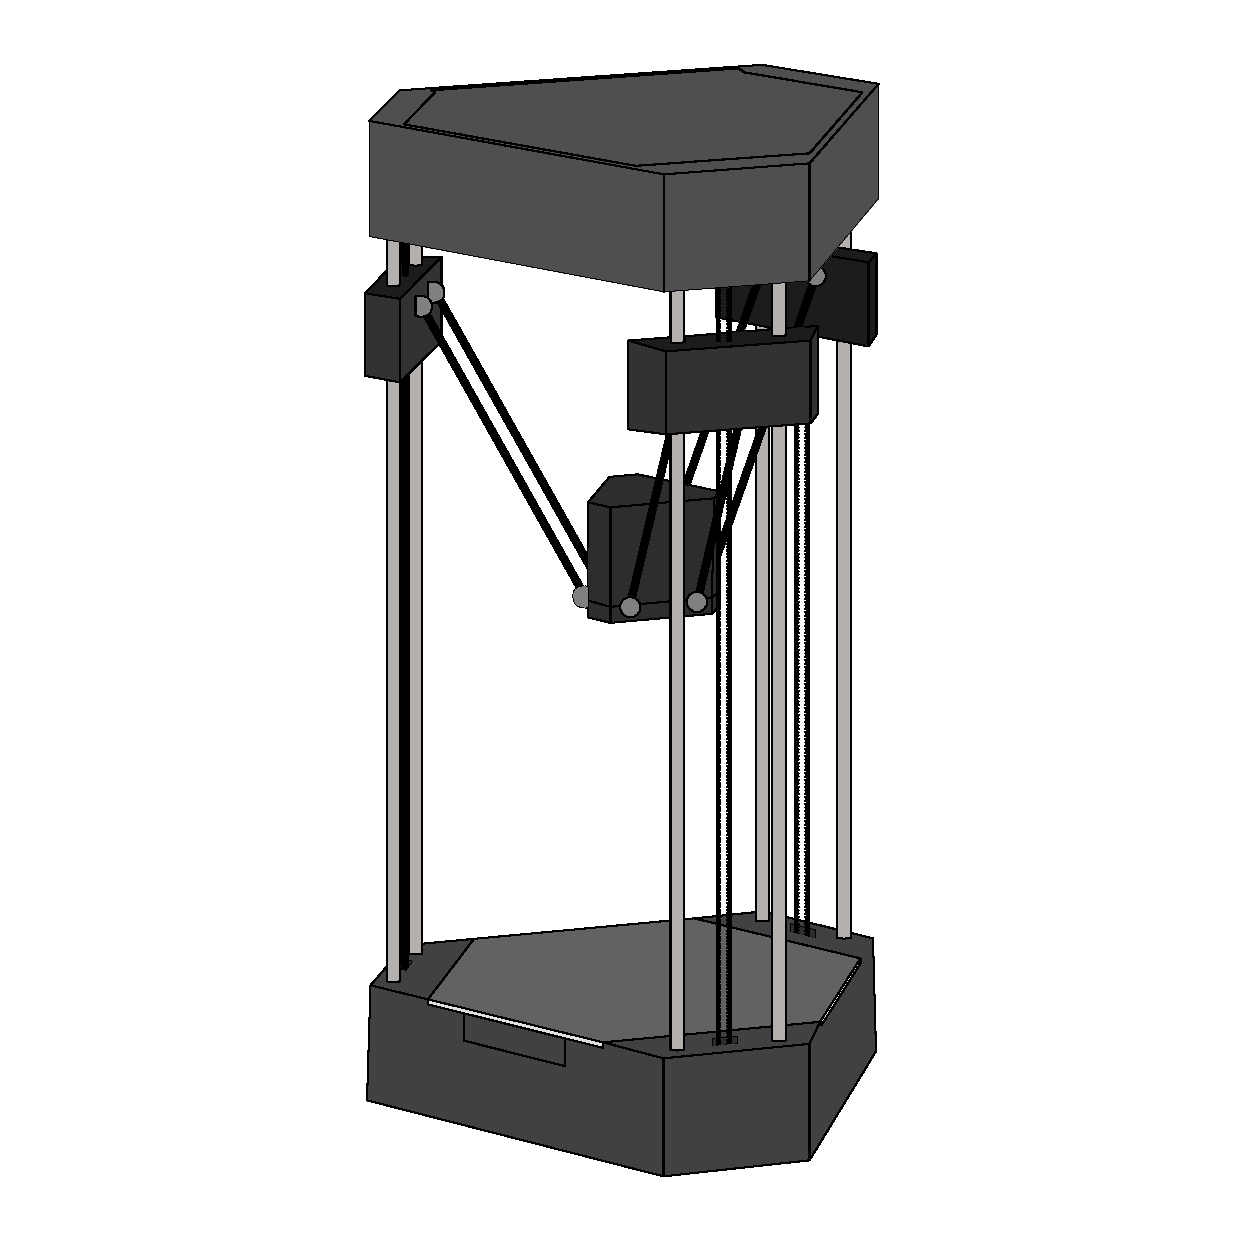
\includegraphics[width=1.0\textwidth, trim = 0px 0px 0px 0px, clip]{./bilder/FLUXX.pdf}
\end{framed}

\end{minipage}}
% \hfill
\adjustbox{valign=t}{\begin{minipage}[t]{0.50\textwidth}
\vspace{0pt}
\huge
\hfill{}\textbf{Flux Delta}
\begin{itemize}
  \item Leveling über Drucksensoren unterhalb des Printbed durch Berührung mit sauberer Düse. 
  \item Bei diesem Modell durch Closed Source Software kein Heatbed möglich.
  \item Delta haben in der Regel ein Bowden Setup
  \subitem Dadurch ist prinzipiell eine hohe Druckgeschwindigkeit möglich.
  \subitem \textbf{ABER}
  \subitem Delta Drucker haben meinstens keinen Partcooler \\ Dadurch sind wiederum nur langsame Geschwindigkeiten Sinnvoll.
\end{itemize}
\end{minipage}}
\end{figure}
\clearpage % GleitObjekte anzeigen

\newpage % ==================================================================


% \subsubsection{Polar}
\begin{figure}[ht]
  \subsubsection{Polar}
  % \section{Sensor - Varianten}
  % \subsection{Andere Ansätze fürs Bedleveling}


\adjustbox{valign=t}{\begin{minipage}[t]{0.45\textwidth}
\begin{framed}
  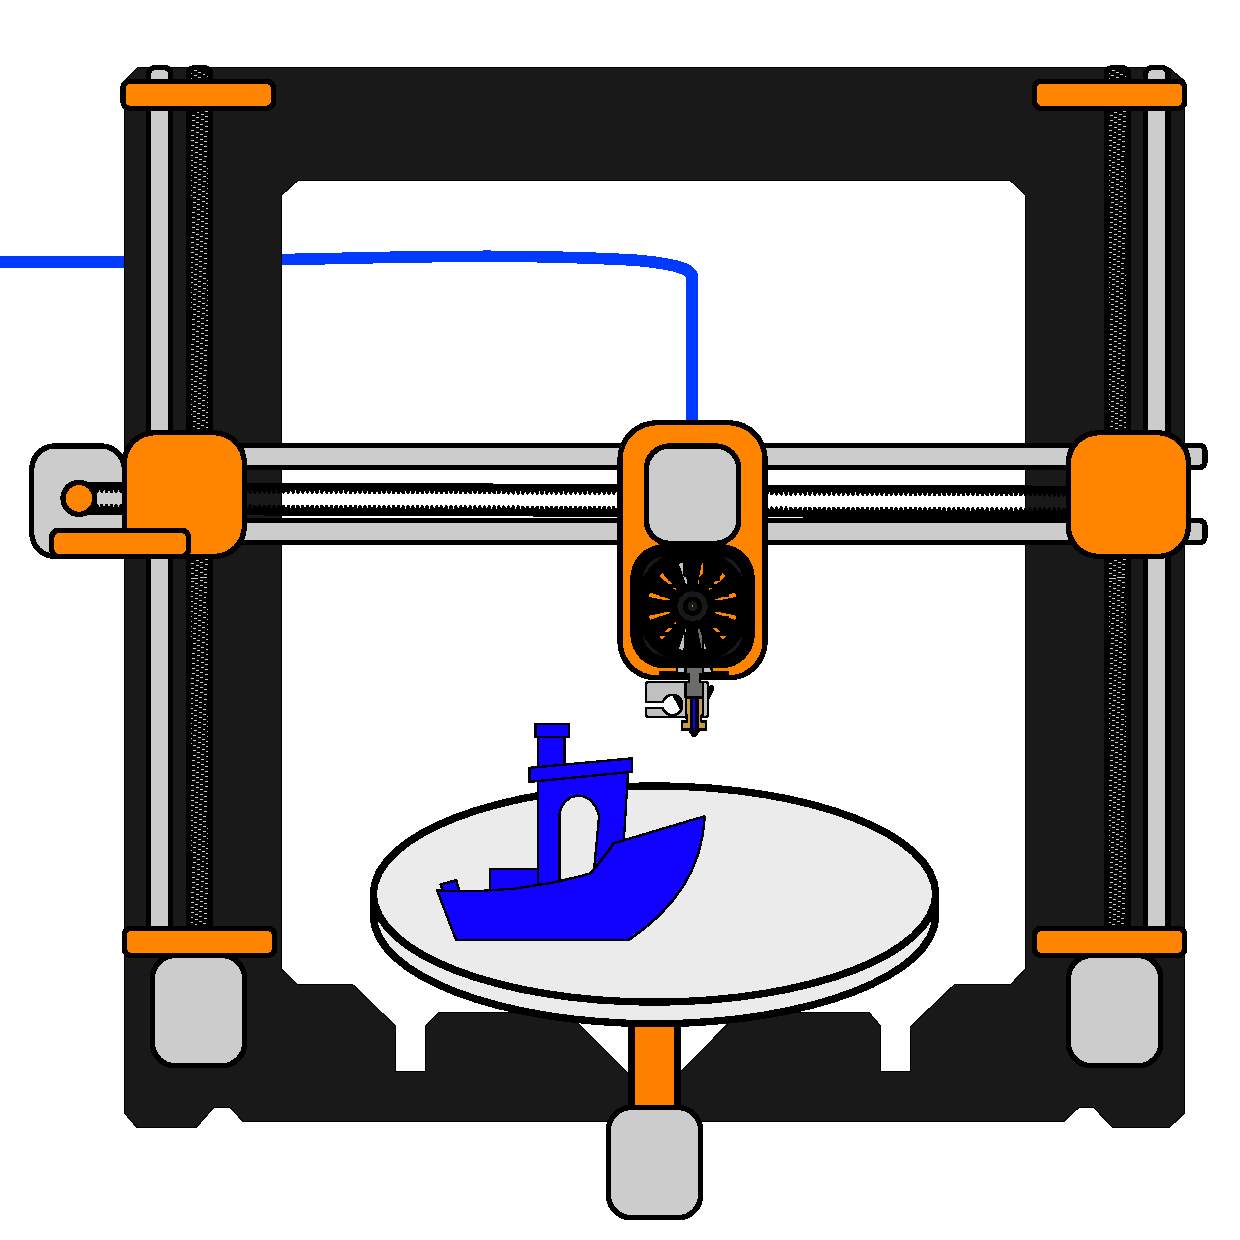
\includegraphics[width=1.0\textwidth, trim = 0px 0px 0px 0px, clip]{./bilder/Polar.pdf}
\end{framed}

\end{minipage}}
% \hfill
\adjustbox{valign=t}{\begin{minipage}[t]{0.50\textwidth}
\vspace{0pt}
\huge
\hfill{}\textbf{Polarer Drucker}\\
\vspace{-0.5cm}
\begin{center}
  \Huge{\textbf{Achtung ab hier nur noch Sarkasmus !!!}}
\end{center}
\textbf{Vorteile:}
\begin{itemize}
  \item Joah !!! \\ Eigentlich nur gut für Vasen.
  \item Man kann 4 Kästen Bier während der Fehlersuche trinken.
  \item Druckbed ist super stabil.
\end{itemize}
\begin{center}
  \Huge{\textbf{Nein, im Ernst einen solchen Drucker sollte man nur bauen wenn man zu viel Zeit hat.}}
\end{center}
% \textbf{Nachteile:}
\end{minipage}}
\end{figure}
\clearpage % GleitObjekte anzeigen

\newpage % ==================================================================

\begin{figure}[ht]
  \subsubsection{HangPrinter}
  % \section{Sensor - Varianten}
  % \subsection{Andere Ansätze fürs Bedleveling}


\adjustbox{valign=t}{\begin{minipage}[t]{0.5\textwidth}
\begin{framed}
  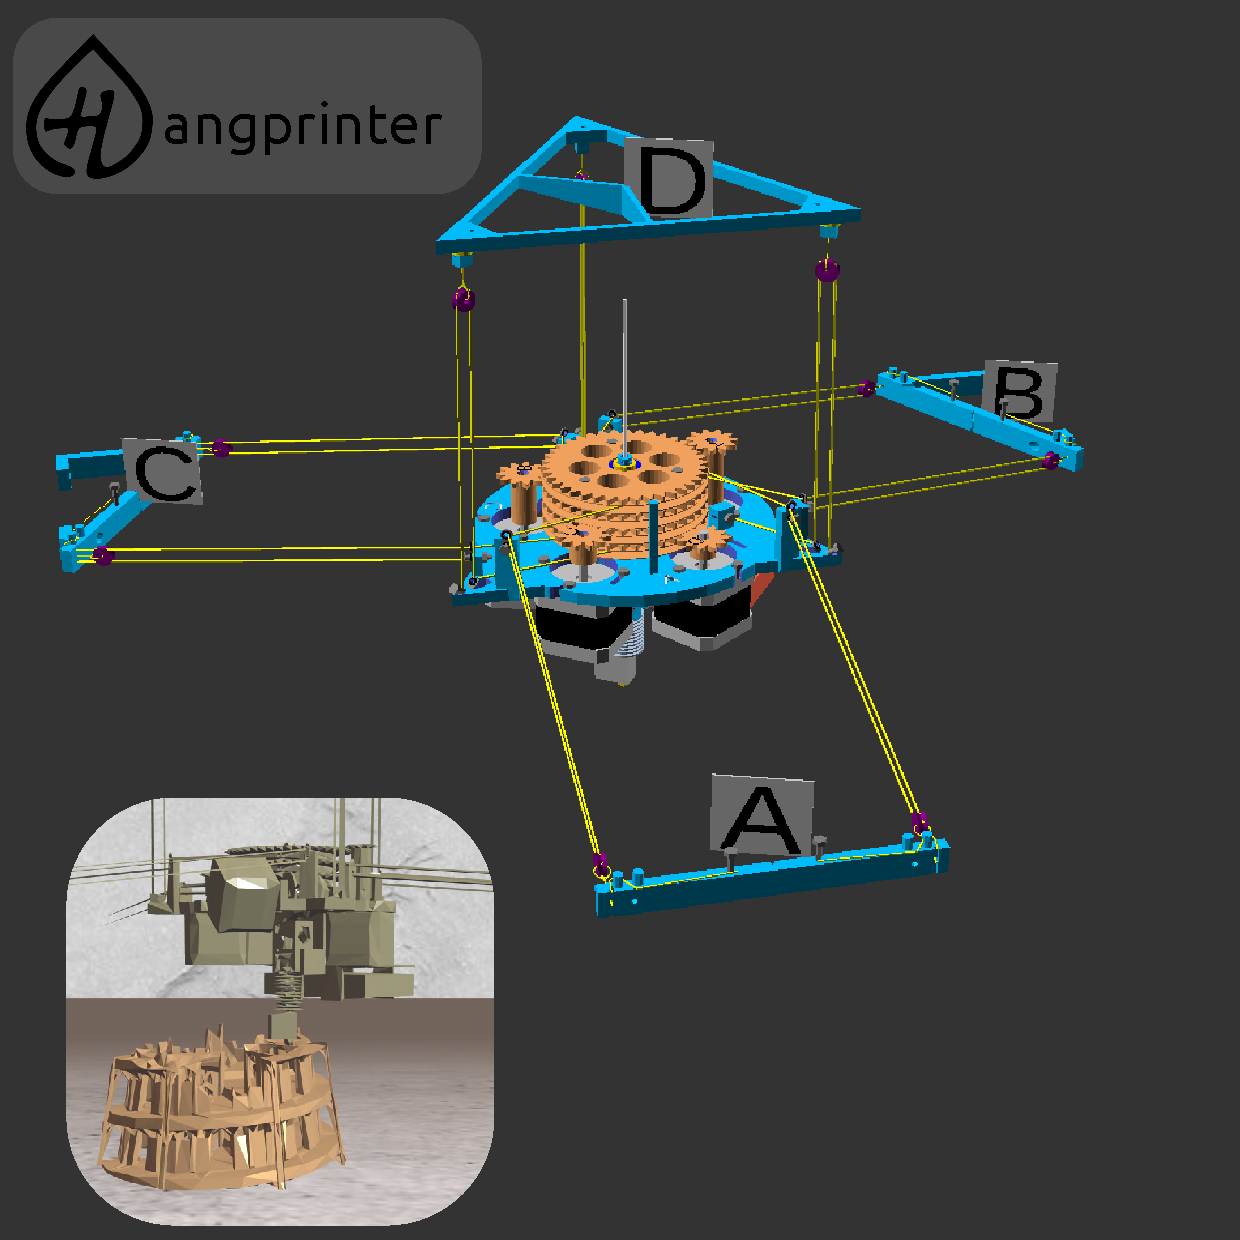
\includegraphics[width=1.0\textwidth, trim = 0px 0px 0px 0px, clip]{./bilder/Hangprinter.pdf}
\end{framed}

\end{minipage}}
% \hfill
\adjustbox{valign=t}{\begin{minipage}[t]{0.45\textwidth}
\vspace{0pt}
\huge
\hfill{}\textbf{HangPrinter}\\
\vspace{-0.5cm}
\begin{center}
  (Spiderman, Spiderman ...)
\end{center}
\vspace{0.2cm}

\textbf{Vorteile:}
\begin{itemize}
  \item Bauraum bis einen die \\ Erdkrümmung kickt.
  \item Keine blöden Bauteile \\ (Wie Gewindestangen, \\Gurte, ...)
\end{itemize}
\textbf{Nachteile:}
\begin{itemize}
  \item Es gibt bisher nur einen.
  \item Relativ wenig doku.
  \item Höchst experimentell.
  \item Nach ca. 1 Meter muss man den Druck pausieren und neu kalibrieren.
\end{itemize}
\end{minipage}}
\end{figure}
\clearpage % GleitObjekte anzeigen

\newpage % ==================================================================





% \vspace{0.5cm}
%
% \begin{center}
%   \includegraphics[width=1.0\textwidth]{./bilder/plainRepo.png}
% \end{center}

%
%
% \begin{figure}[]
%   \subsubsection{Github Repo mit Travis CI verbinden}
% \adjustbox{valign=t}{\begin{minipage}[t]{0.50\textwidth}
% \begin{framed}
%   \includegraphics[width=1.0\textwidth]{./bilder/1gitRepoSettings.png}
% \end{framed}
%
% \end{minipage}}
% % \hfill
% \adjustbox{valign=t}{\begin{minipage}[t]{0.5\textwidth}
% \vspace{0pt}
% \huge
% Im Repo klickt man auf Settings
% % \caption{Kapazität}
% \end{minipage}}
% % \end{figure}
% % \vspace{0.5cm} % ----------------------------------- vspace
% % \begin{figure}[ht]
% \adjustbox{valign=t}{\begin{minipage}[t]{0.40\textwidth}
% % \vspace{0.5cm}
% \begin{framed}
%   \includegraphics[width=1.0\textwidth]{./bilder/2integrationServices.png}
% \end{framed}
%
% \end{minipage}}
% \hfill
% \adjustbox{valign=t}{\begin{minipage}[t]{0.43\textwidth}
% \vspace{0pt}
% \huge
% Danach
% % \caption{Kapazität}
% \end{minipage}}
% \end{figure}
%
% \clearpage % GleitObjekte anzeigen
% \newpage
% \begin{table}
%   \caption{title}
% \end{table}
% Test


% \begin{center}
%  % \includegraphics[scale=0.5]{./pictures/wohnzimmer.png}
% \end{center}
% \begin{figure}
%     \subfigure[Bezeichnung der linken Grafik]{\includegraphics[width=0.49\textwidth]{./bilder/1gitRepoSettings.png}}
%     \subfigure[Bezeichnung der rechten Grafik]{\includegraphics[width=0.49\textwidth]{./bilder/2integrationServices.png}}
% \caption{Titel unterm gesamten Bild}
% \end{figure}


% \begin{figure}
%     \subfigure[Bezeichnung der linken Grafik]{\includegraphics[width=0.49\textwidth]{./bilder/1gitRepoSettings.png}}
%     \subfigure[Bezeichnung der rechten Grafik]{Test tesxt}
% \caption{Titel unterm gesamten Bild}
% \end{figure}


%
% \section{Bauformen von 3D Druckern}
% as
% \subsection{Drucker nach Materialart}
% as
% \subsubsection{SLA}
% asas
% \subsubsection{FDM}
% asasas
% \subsection{Bauformen von FDM Druckern}
% \subsubsection{Karthesisch}
% \subsubsection{CoreXYZ}
% \subsubsection{Delta}
% \subsubsection{Hangprinter}
% \subsubsection{rotierend}
